\chapter{提案: ユーザレビューの分析および開発者支援ツール}
\label{chap:teian}

%ーーーーーーーーーーーーーーーーーーーーーーーーーーーー

\section{概要}
既存研究の多くはカテゴリやトピックを事前に定義した上で分類している. したがって, レビューの特徴に応じてトピックやカテゴリを変更することができないため, ``アプリの欠陥''や``賞賛''といった粒度の粗いクラスタリングとなってしまう. 
また, 既存研究の多くは, トピック分類やキーワード抽出を実行した結果を示すところまでしか提案されていない. したがって, マイニングによって得られた結果を利用して, 開発者やユーザを支援するようなツールは提案されていない. 

したがって本論文では, レビューに含まれる開発に有用な情報 (アプリの欠陥やアプリに対する要望) を示す箇所 (以下 : キーフレーズ) のみを抽出し, キーフレーズを内容に応じてクラスタリングすることにより粒度の細かいクラスタリング手法を提案する. 
また, その結果をwebブラウザ上で表示し, 開発者がレビューの閲覧, 分析をしやすくする開発者支援ツールを提案する. 

\section{提案手法の流れ}
本研究で提案している手法やツールの流れを下記に示す. 

\begin{enumerate}
  \item Google PlayストアとTwitterに投稿されたレビュー及びツイートをスクレイピングして取得, 前処理
  \item キーフレーズを自動抽出
  \item 抽出したキーフレーズを利用しクラスタリング
  \item マイニングした結果をwebブラウザ上で可視化
\end{enumerate}

提案手法の流れを図\ref{fig:nagare}に示す. 

\begin{figure}[H]
  \centering
  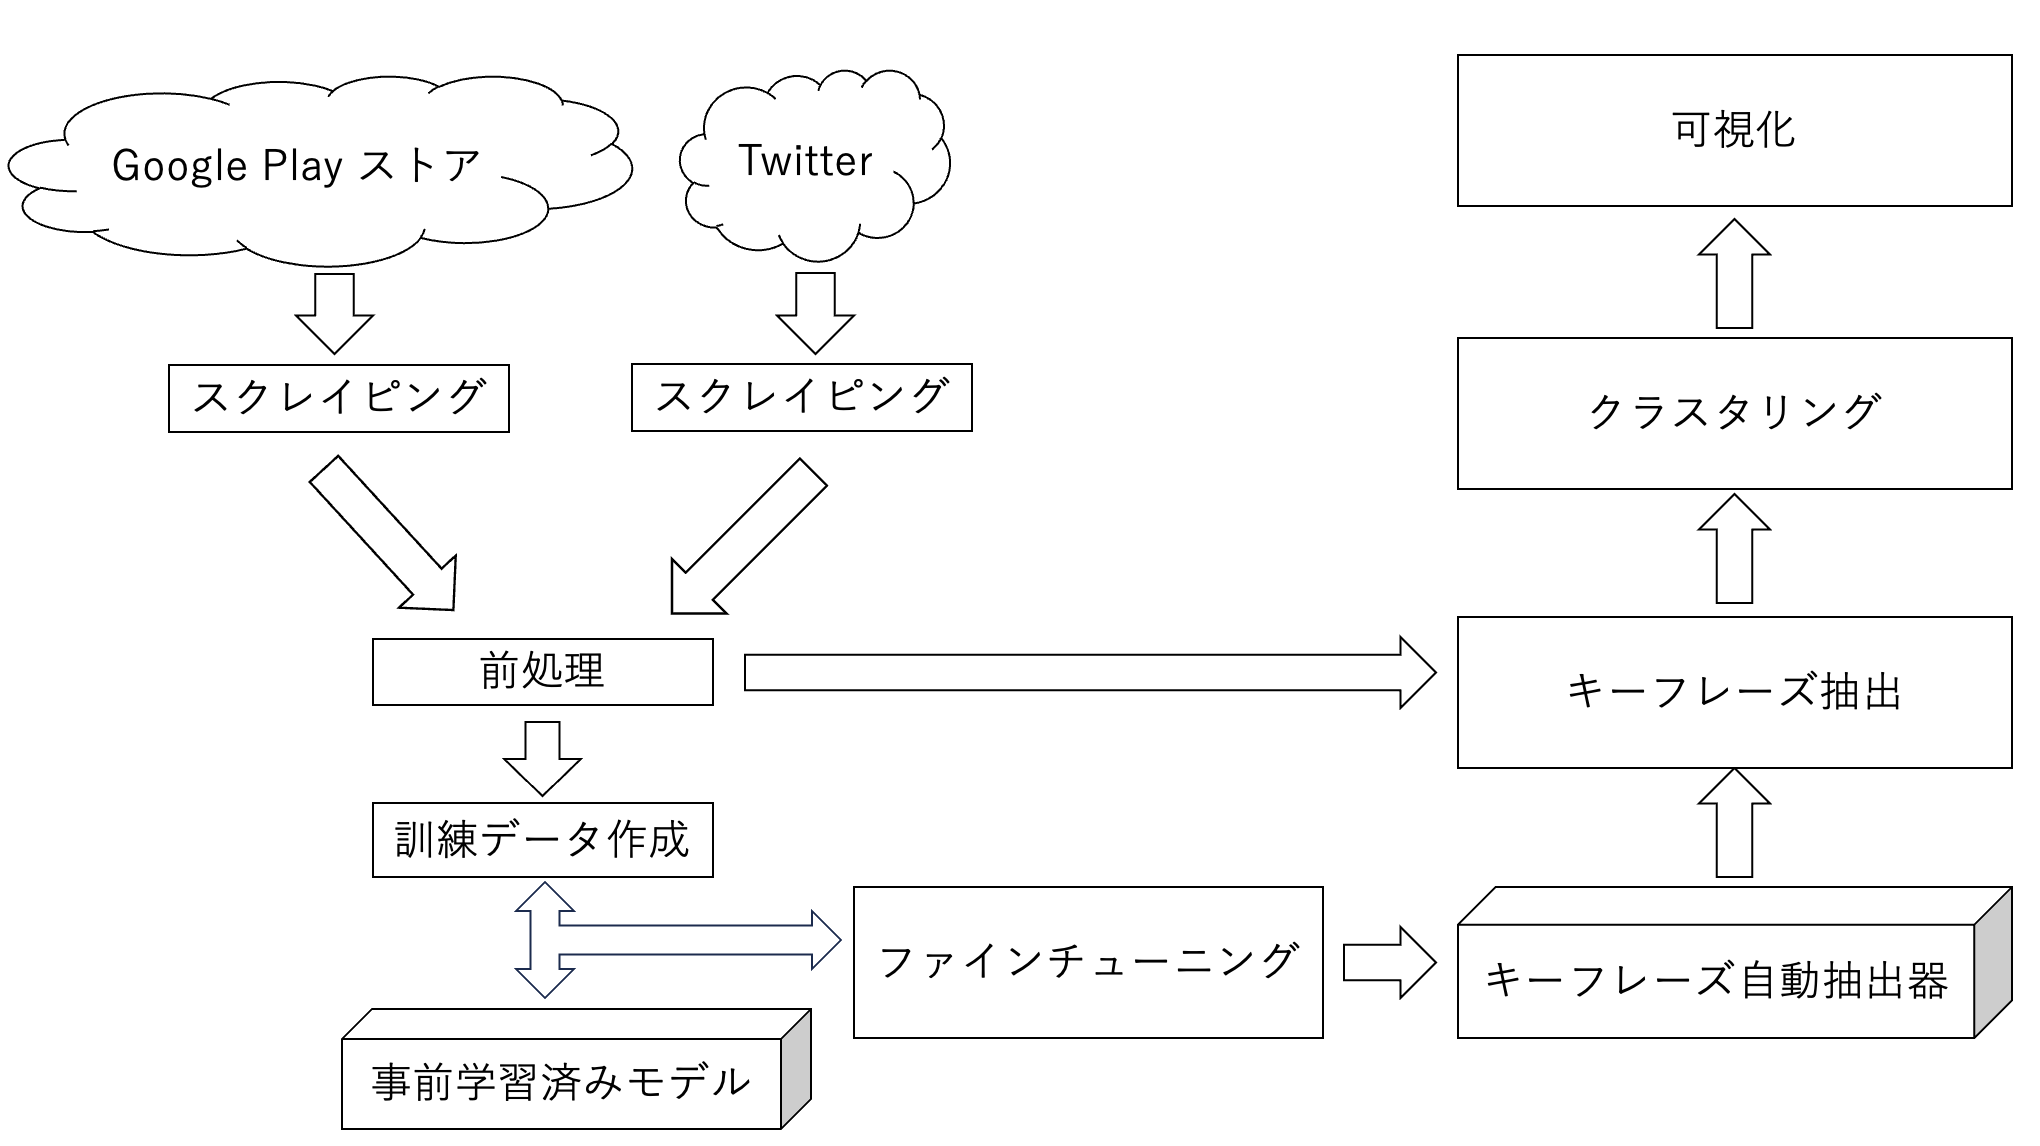
\includegraphics[scale=0.35]
    {contents/images/zisso.png}
  \caption{実装した提案手法の流れ\label{fig:nagare}}
\end{figure}

図\ref{fig:nagare}の各処理に関して, 実装の詳細を説明している節は次に示す通りである. 

\begin{itemize}
  \item Google PlayストアとTwitterからのスクレイピング: \ref{scraping}節
  \item スクレイピングされた情報の前処理: \ref{preprocessing}節
  \item 自動抽出: \ref{extraction}節
  \item クラスタリング: \ref{clustering}節
  \item 可視化: \ref{display}節
\end{itemize}

%ーーーーーーーーーーーーーーーーーーーーーーーーーーーー

\section{対象アプリとレビュー}
本研究では川面による先行研究\cite{kawatsura}のデータセットを使用するため対象アプリは先行研究のアプリに合わせている. 注意点として, BuzzVideoは2022年3月をもってサービスを終了しているため, 本研究で新たに取得するレビューの対象となるアプリはBuzzVideo以外の12個のアプリである. 
対象となっているアプリを表\ref{tb:taisyouapuri}に示す. 
\begin{table}[H]
  \small
  \caption{本研究の対象アプリ一覧}
  \label{tb:taisyouapuri}
  \begin{center}
  \begin{tabularx}{\linewidth}{l|l|X}
    \hline
    \mbox{アプリ名}\mbox{(一部略称)}&\mbox{Google Playストアの}\mbox{パッケージID}&\mbox{Twitterの}\mbox{検索キーワード}\\\hline\hline
    にゃんトーク&com.akvelon.meowtalk&にゃんトーク\\\hline
    スマートニュース&jp.gocro.smartnews.android&スマートニュース\\\hline
    PayPay&jp.ne.paypay.android.app&paypay\\\hline
    Coke ON&com.coke.cokeon&coke on\\\hline
    Google Fit&com.google.android.apps.fitness&google fit\\\hline
    Simeji&com.adamrocker.android.input.simeji&simeji\\\hline
    Lemon8&com.bd.nproject&lemon8\\\hline
    楽天ペイ&jp.co.rakuten.pay&楽天ペイ\\\hline
    majica&com.donki.majica&majica\\\hline
    LINE MUSIC&jp.linecorp.linemusic.android&line music\\\hline
    BuzzVideo&com.ss.android.article.topbuzzvideo&buzzvideo\\\hline
    ファミペイ&jp.co.family.familymart\verb|_|app&ファミペイ\\\hline
    CapCut&com.lemon.lvoverseas&capcut\\\hline
  \end{tabularx}\end{center}
\end{table}

%ーーーーーーーーーーーーーーーーーーーーーーーーーーーー

\section{スクレイピング・前処理}
本研究で対象としているアプリに関するGoogle PlayストアとTwitterのレビュー及びツイートをスクレイピングし, 分析対象となるデータセットを作成する. このデータセットは, 先行研究で作成された13個のアプリに関するレビューのデータセットと, 本研究で作成した12個のアプリに関するレビューのデータセットの2つで構成されている. 
対象アプリを先行研究に合わせた理由としては, 現在, Twitterの利用規約によりツイートの収集可能な数に制限がある影響で, 本研究だけでは十分な数のツイートが収集できなかったためである. Twitterのツイート取得数に関する制限の詳細は\ref{sec:x}項で後述する. 
データセットからキーフレーズを自動抽出するために一般的な自然言語処理で行われる前処理を行う. 

%ーーーーーーーーーーーーーーーーーーーーーーーーーーーー

\section{キーフレーズの自動抽出}
\subsection{概要}
本研究におけるキーフレーズの自動抽出における役割は次に示す2つである. 
\begin{itemize}
  \item 前処理された大量のレビューからキーフレーズが記述されているレビューのみを絞り込む
  \item レビューからキーフレーズを抽出する
\end{itemize}
これによりアプリの欠陥やアプリに対する新たな機能の要望など開発に有用な情報のみが取得できる. 

\subsection{使用するモデル}
日本語のデータで事前学習済みの言語表現モデルである日本語BERTに対して質問応答形式のファインチューニングを行うことで自動抽出モデルを生成する. 
図\ref{fig:fine-tuning}に質問応答形式によるファインチューニングのモデルを示す. 

\begin{figure}[H]
  \centering
  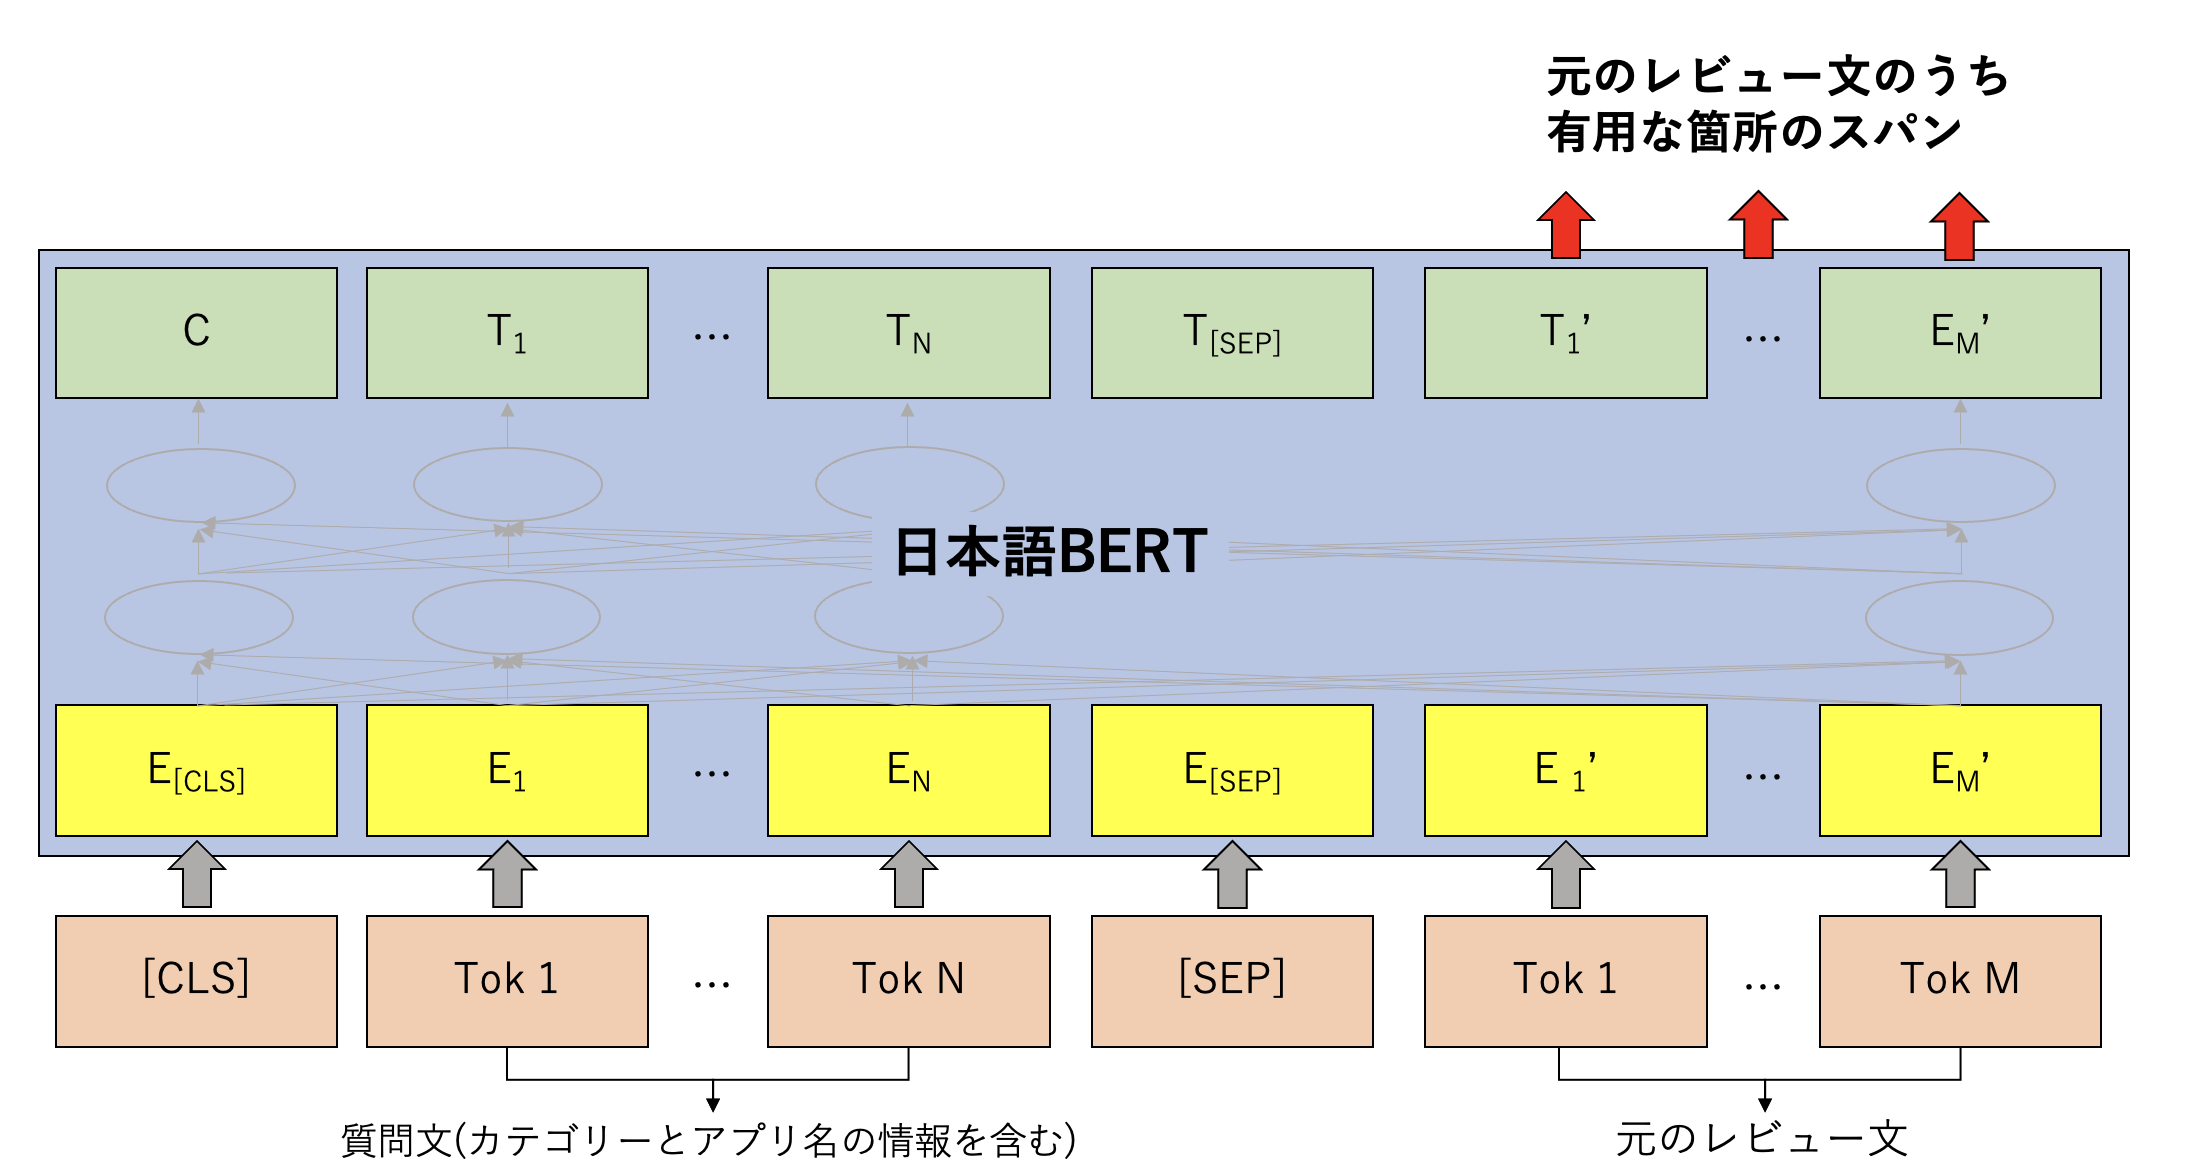
\includegraphics[scale=0.3]
    {contents/images/fine-tuning.png}
  \caption{質問応答形式によるファインチューニングのモデル\label{fig:fine-tuning}}
\end{figure}
\noindent
図\ref{fig:fine-tuning}で示したファインチューニングには元のレビューとアプリの欠陥や要望を尋ねる質問文, 抽出したいキーフレーズの3つの情報を含めたQA用データセットが必要となる. データセットの詳細は\ref{dataset}項で後述する. 
QA用データセットを使用してファインチューニングを実行することで, アプリの欠陥や要望を尋ねる質問に対して元のレビューからキーフレーズを抽出するモデルを生成する. 
抽出対象となる元のレビューの特徴をモデルに理解させるために質問文にその文章がGoogle PlayストアのレビューなのかTwitterのツイートなのかという``カテゴリー''の情報と``アプリ名''の情報を加えることにより学習性能を上げる. 

図\ref{fig:answer}に元のレビューと質問文, キーフレーズの組み合わせの例を示す. 質問文がアプリの欠陥やアプリに対する要望を尋ねる文章となっており, その答えが元のレビューから抽出するキーフレーズとなっている. 

\begin{figure}[H]
  \centering
  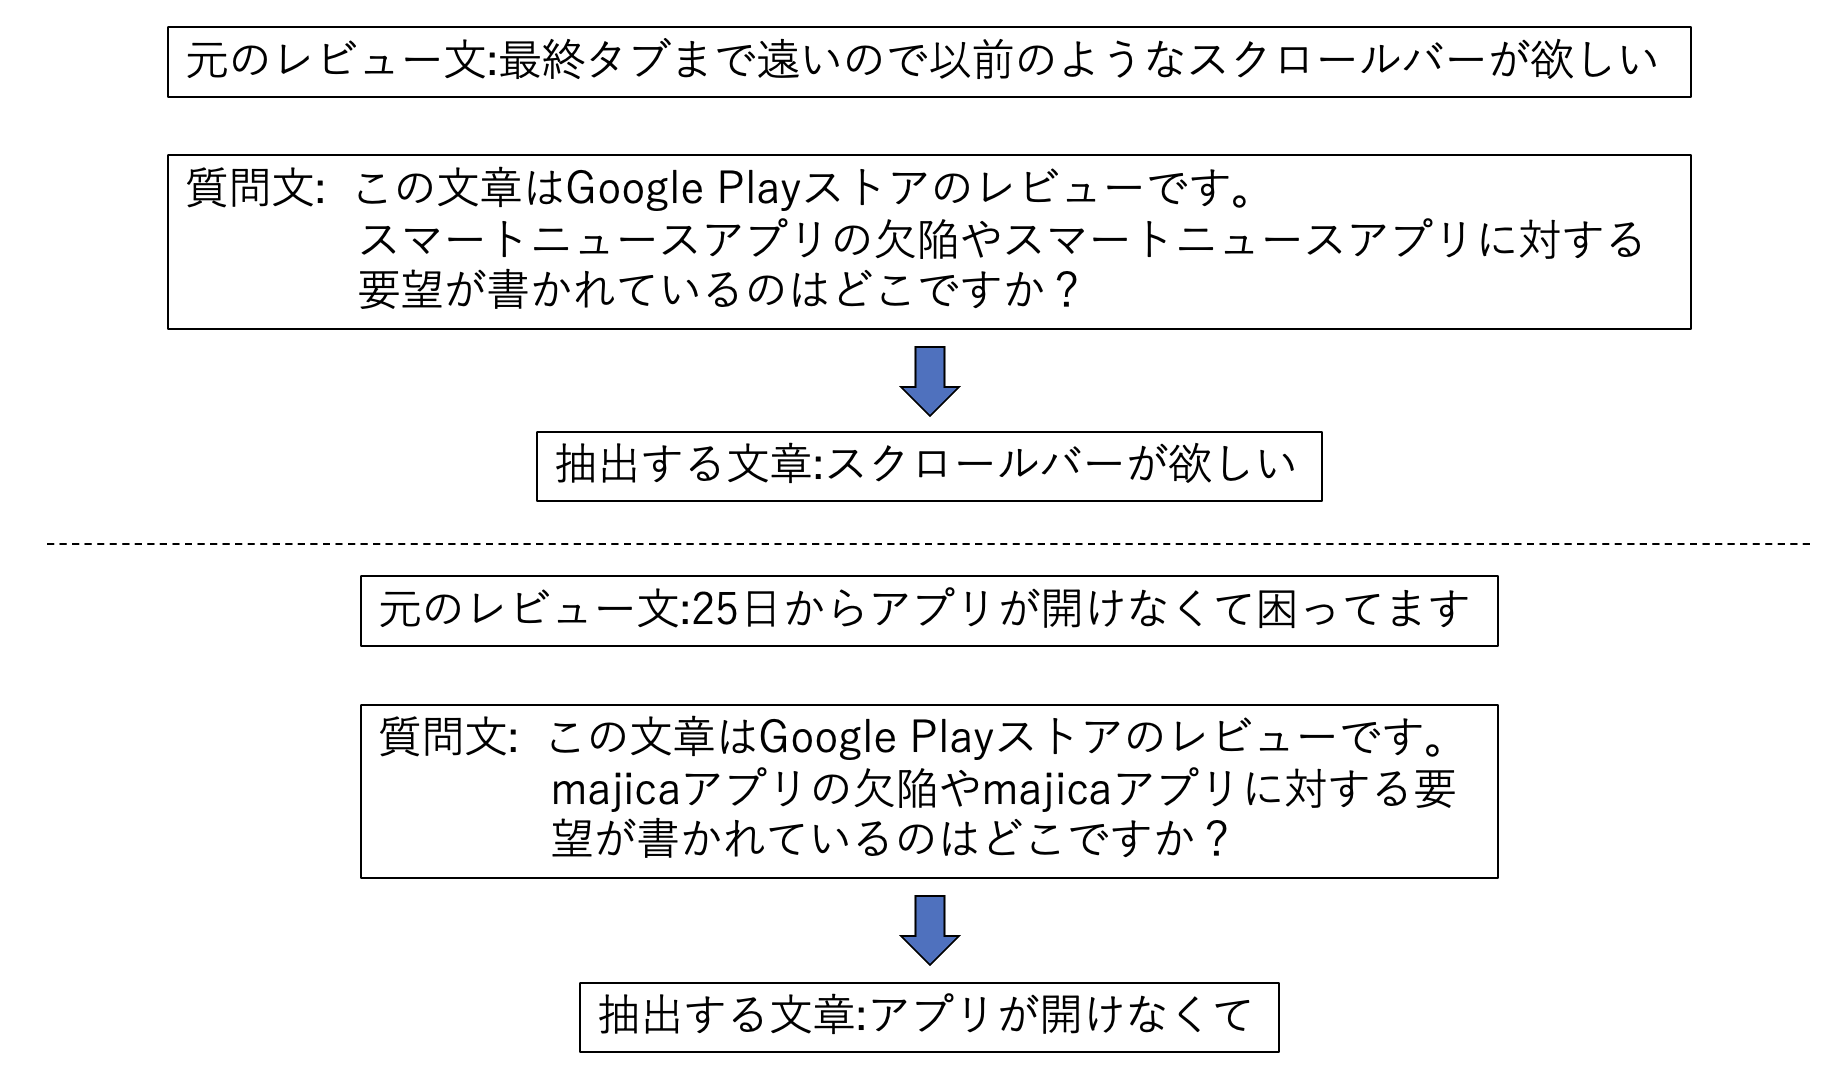
\includegraphics[scale=0.4]
       {contents/images/answer.png}
  \caption{キーフレーズの抽出例\label{fig:answer}}
\end{figure}

%ーーーーーーーーーーーーーーーーーーーーーーーーーーーー

\section{クラスタリング}
\subsection{概要}
本研究におけるクラスタリングの役割は次に示す2つである. 
\begin{itemize}
  \item 抽出された各キーフレーズを類似度に応じてクラスタリングする
  \item それぞれのクラスタの特徴を表す名称 (以下 : クラスタ名) を決める
\end{itemize}

\subsection{クラスタリング手法}\label{graph_clustering}
抽出したキーフレーズのクラスタリングにはChinese Whispers\cite{chinese-whispers}というグラフクラスタリング手法を使用する. グラフ作成のために抽出したキーフレーズをSentence-BERTの日本語モデルによってベクトルに変換する. Sentence-BERT\cite{sentence-bert}とは, 事前学習されたBERTモデルとSiamese Networkを使い, 高品質な文ベクトルを作る手法である. 
したがって本研究でのクラスタリング手法は下記の手順である. 
\begin{enumerate}
  \item Sentence-BERTの日本語モデルを用いて, 抽出した文章をベクトルに変換
  \item 重み付き無向グラフを構成し, 抽出したキーフレーズをノードとし, 2つのノード間のコサイン類似度スコアをノード間の重みとする. スコアがある閾値以上の場合, 2つのノード間にエッジを追加. この閾値は入力ハイパーパラメータであり, 抽出されたキーフレーズ間の意味的相関を測定するために使用される. 閾値が高いほどクラスタの結束力が高まる. 
  \item このグラフに対して, Chinese Whispersを実行し, 抽出したキーフレーズをクラスタリング. 
\end{enumerate}

図\ref{fig:clustering}にクラスタリングの概略図を示す. 丸で示されているのが抽出されたキーフレーズを表すノードであり, 点線がエッジである. このエッジは設定された閾値によって変化する. 
\begin{figure}[H]
  \centering
  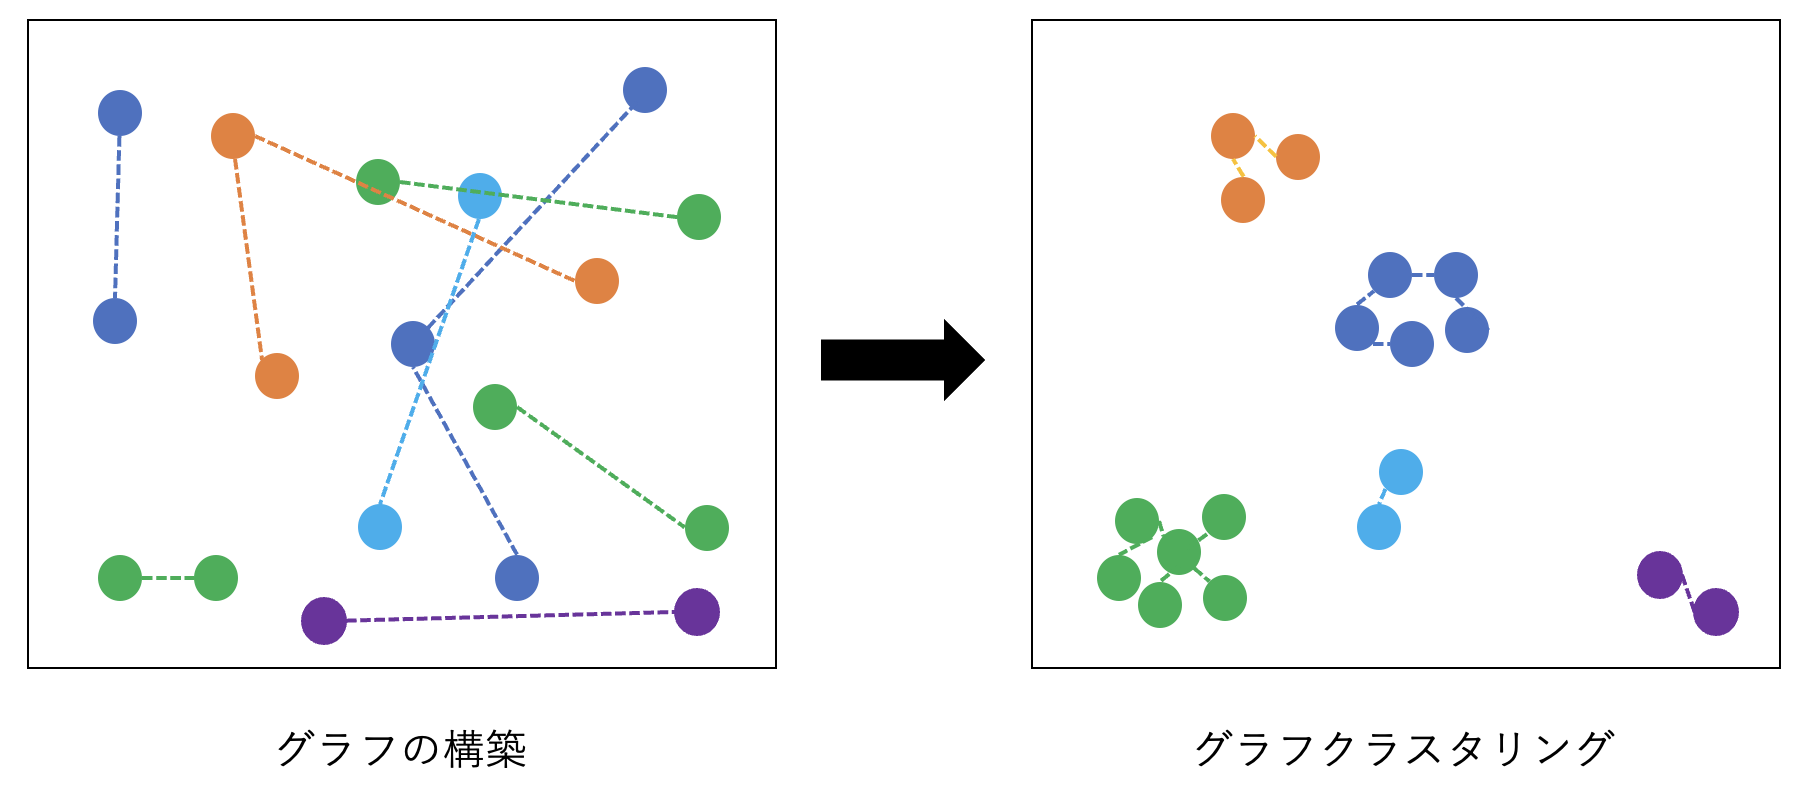
\includegraphics[scale=0.4]
       {contents/images/clustering.png}
  \caption{グラフクラスタリングの概略図\label{fig:clustering}}
\end{figure}

\subsection{クラスタ名の決定}
クラスタを作成したら各クラスタのクラスタ名を決定する. 
クラスタ名の決定にはKeyBERT\cite{keybert}を使用したキーワードの抽出によって実現する. KeyBERTとは, BERTの埋め込みを活用して, 文書に最も類似したキーワードを作成するキーワード抽出技法である. 
具体的な手順は次に示す通りである. 

\begin{enumerate}
  \item 文書レベルの表現を得るために, BERTを用いて文書埋め込みを抽出する
  \item N-gramの単語やフレーズについて単語埋め込みを抽出する
  \item コサイン類似度を用いて, 文書に最も類似する単語を見つける. 最も類似している単語は, 文書全体を最もよく表現する単語として特定される
\end{enumerate}

%ーーーーーーーーーーーーーーーーーーーーーーーーーーーー

\section{可視化}
マイニングした結果を用いてwebブラウザ上で可視化を行う. クラスタごとにまとめて表示することで, 開発者は類似した内容のレビューをまとめて確認できる. 
開発者はアプリの修正やアップデートを行った後に, ユーザがどのようなレビューを挙げているかを特に確認したいと考えられる. したがって, 特定の機能や期間でのレビュー内容を確認できるよう, レビューが投稿された期間やキーワードで絞り込むことが可能な検索機能を実装した. 
そして, レビューの特徴を確認するために次に示す2つのグラフを実装した.
\begin{itemize}
  \item 日ごとのレビュー数を表す折れ線グラフ
  \item クラスタに含まれるレビュー数の上位10個を表す棒グラフ
\end{itemize}
日ごとのレビュー数の推移を表す折れ線グラフによって, どの期間に多くレビューが投稿されたかをすぐに確認することができる. そのため, 開発者はその期間のレビューを集中的に確認, 分析することが可能となる. 
また, クラスタに含まれるレビュー数の上位10個を表す棒グラフによって, そのアプリにはどのような種類のレビューが多く投稿されているのか, レビューの傾向などを理解しやすいようになっている. 
そして, この2つのグラフは検索結果に対応して変化するようになっている. 
レビューをクラスタごとに表示するだけでなく, 検索機能を実装しグラフを表示することで, 開発者がレビューを理解, 分析しやすいツールとなっている. 